\documentclass[aspectratio=169]{beamer}
\usepackage{lmodern}
%\usetheme{Madrid}
%\usecolortheme{giantoak}
\newcommand*\oldmacro{}
\let\oldmacro\insertshorttitle
\renewcommand*\insertshorttitle{\oldmacro\hfill\insertframenumber\,/\,\inserttotalframenumber}
\usepackage[framemethod=tikz]{mdframed}

%\usepackage{beamerthemesplit}
\usepackage{textpos}
\usepackage{pgf}
%\logo{\pgfputat{\pgfxy(0,-.4)}{\pgfbox[right,base]{\includegraphics[height=1.0cm]{logo.jpg}}}}
%\newcommand{\nologo}{\setbeamertemplate{logo}{}}
\usepackage{booktabs}
\usepackage{graphicx}
\theoremstyle{principle}
\newtheorem*{principle}{Design Principle}


\titlegraphic{\includegraphics[width=1.0\paperwidth]{cool-wind-800px.jpg}}

\title{What even is `science?'}
%\author[Jeremy Kedziora]{Wind Data Science Team\\
%\small{Uptake}}
\date{}

\begin{document}

%{
%%\nologo
%\begin{frame}
%    \maketitle
%\end{frame}
%}
%pages 1-7, 8-9, 14-15.


{
%  \usebackgroundtemplate{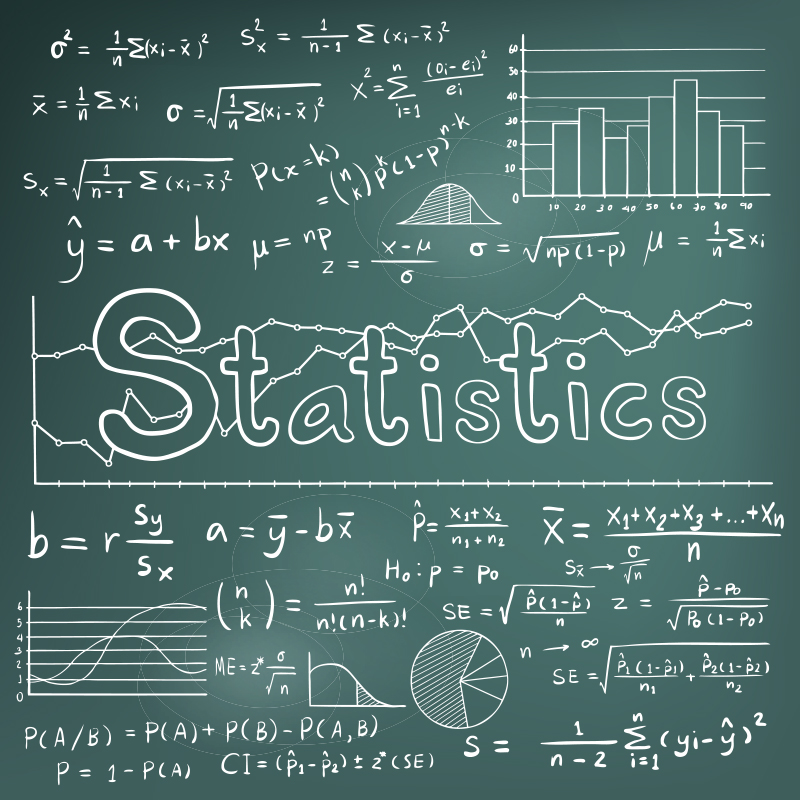
\includegraphics[width=1.0\paperwidth]{statistics-review.jpg}}
  \usebackgroundtemplate{
\includegraphics[scale=0.8]{science.png}}
  \begin{frame}[plain]
  
\begin{mdframed}[tikzsetting={draw=white,fill=white,fill opacity=0.6,draw opacity=0.4,
               line width=0pt},backgroundcolor=none,leftmargin=20,
               rightmargin=20,innertopmargin=4pt]
\begin{center}
\Huge \textbf{What even is `science?'}
\end{center}
\end{mdframed}

  \end{frame}
}

%@@@@@@@@@@@@@@@@@@@@@@@@@@@@@@@@@@@@@@@@@@@@@@@@@
\begin{frame}
\frametitle{Today:}
\begin{itemize}
\item What is `science';
\bigskip
\bigskip
\bigskip
\item Theory, hypothesis, implication, test;
\bigskip
\bigskip
\bigskip
\item The underlying logic of science.
\end{itemize}

\end{frame}


%@@@@@@@@@@@@@@@@@@@@@@@@@@@@@@@@@@@@@@@@@@@@@@@@@
\begin{frame}
\frametitle{What science is NOT...}
\begin{itemize}
\item Just a collection of facts;
\bigskip
\item A mechanistic process;
\bigskip
\item A single technical method (e.g. hypothesis testing);
\bigskip
\item A topic (e.g. physics);
\bigskip
\item Technology or engineering;
\bigskip
\item A framework for making moral, aesthetic, or normative judgements;
\bigskip
\item Truth.
\end{itemize}

\end{frame}

%@@@@@@@@@@@@@@@@@@@@@@@@@@@@@@@@@@@@@@@@@@@@@@@@@
\begin{frame}
\frametitle{Ok, then so what is science?  Lots of views...}

\begin{columns}
\begin{column}{0.5\textwidth}

\begin{itemize}
\item \textbf{Rationalism}: theory generated deductively via reason $\Rightarrow$ knowledge;
\bigskip
\bigskip
\item \textbf{Empiricism}: observation $\Rightarrow$ knowledge $\Rightarrow$ general theory;
\bigskip
\bigskip
\item \textbf{Critical rationalism}: theory $\Rightarrow$ \textbf{falsifiable} hypotheses and tests $\Rightarrow$ knowledge.
%\bigskip
%\item Constructive empiricism: Theory $\Rightarrow$ hypotheses about observables which, if true $\Rightarrow$ knowledge.
\end{itemize}

\end{column}
\begin{column}{0.5\textwidth}

\includegraphics[scale=0.4]{experiment.png}
\end{column}
\end{columns}
\end{frame}

%@@@@@@@@@@@@@@@@@@@@@@@@@@@@@@@@@@@@@@@@@@@@@@@@@
\begin{frame}
\frametitle{Ok, then so what is science? My perspective:}
\begin{center}
\Large \textbf{Science = the iterative interplay between theory and empirical observation with the goal to produce an ever-better approximation of the world.}
\end{center}
\end{frame}

%%@@@@@@@@@@@@@@@@@@@@@@@@@@@@@@@@@@@@@@@@@@@@@@@@@
%\begin{frame}
%\frametitle{Choices}
%\begin{center}
%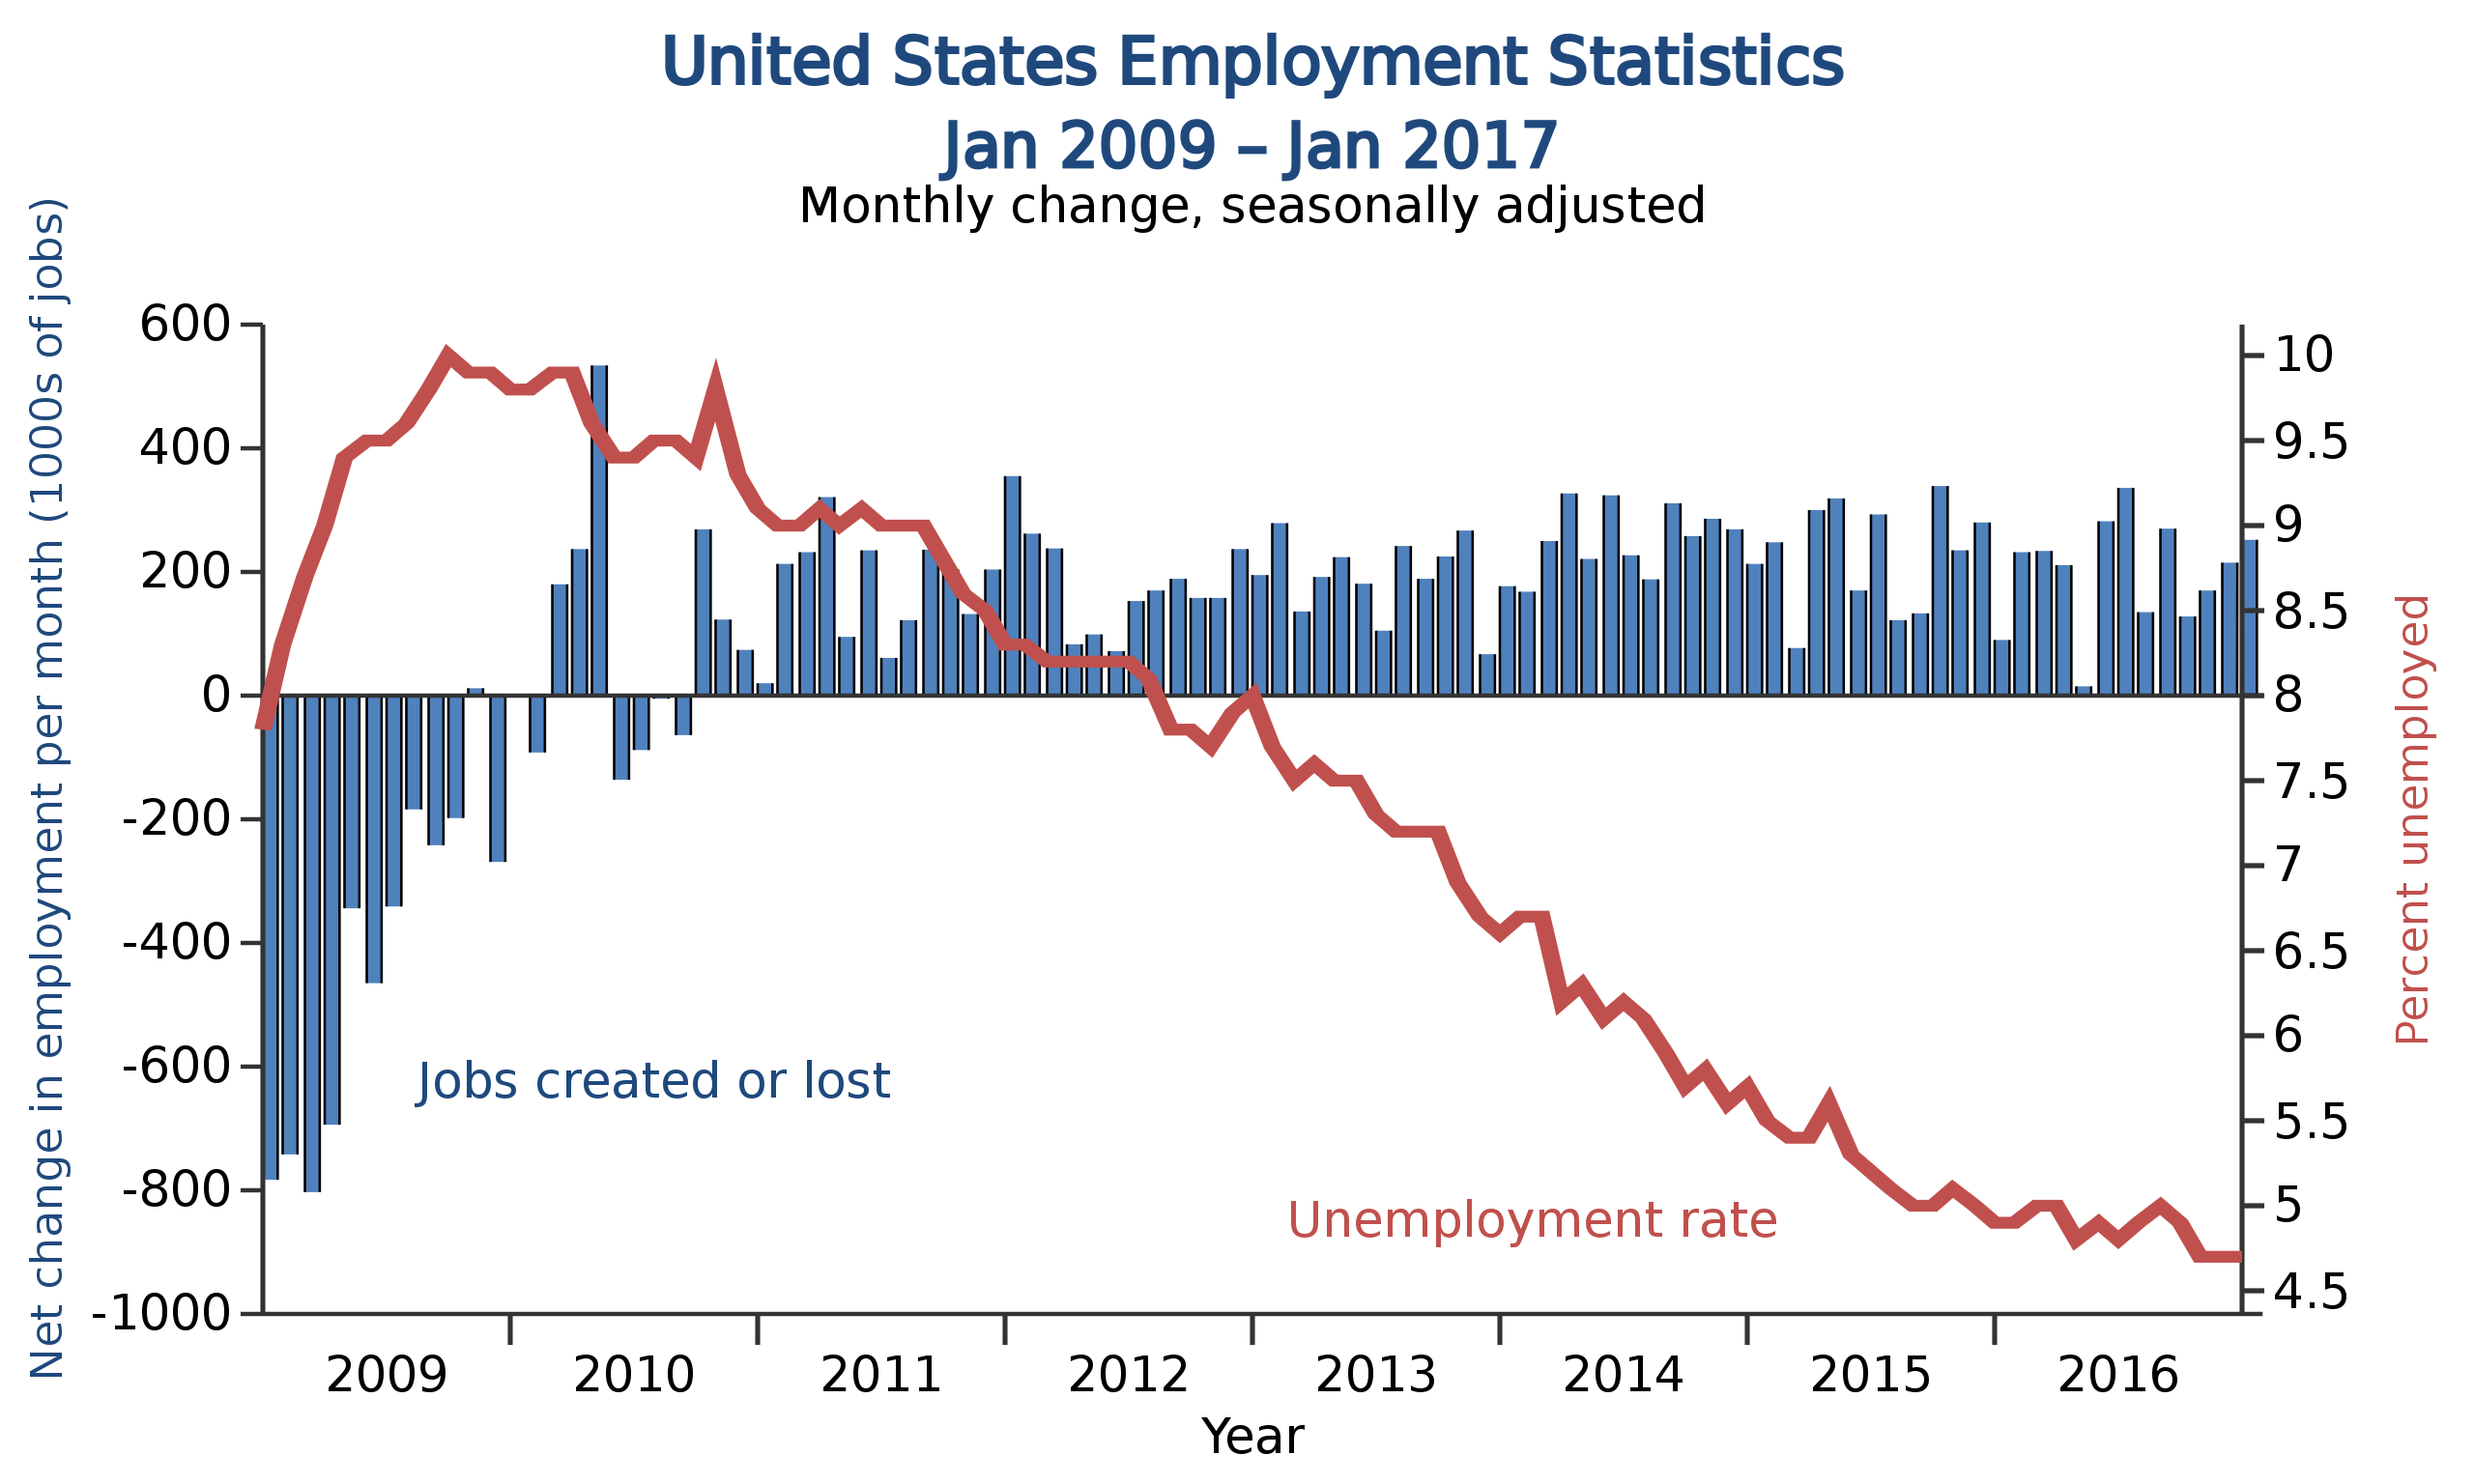
\includegraphics[scale=0.12]{unemployment.png}
%\end{center}
%
%\end{frame}

%@@@@@@@@@@@@@@@@@@@@@@@@@@@@@@@@@@@@@@@@@@@@@@@@@
\begin{frame}
\frametitle{Expanding this...}
\begin{itemize}
\item \textbf{Theory};
\begin{itemize}
\item Characteristics: 
\begin{itemize}
\item Explains; 
\item Characterizes empirical phenomena as generated by underlying processes governed by theoretical first principles; predicts new empirical regularities;
\item Contains `bridge principles' that connect unobservable processes to observables;
\end{itemize}
\item Example: The Theory of Relativity, Spatial Voting;
\end{itemize}
\bigskip
\item \textbf{Empirical Observation};
\begin{itemize}
\item Characteristics: 
\begin{itemize}
\item Information accessible to observation, e.g. sense experience or measurement procedure;
\item Adjudicates between competing potential theories;
\end{itemize}
\item Example: Data on legislative roll calls in the US congress;
\end{itemize}
\bigskip
\item \textbf{Law};
\begin{itemize}
\item Characteristics: 
\begin{itemize}
\item Describes;
\item Asserts a uniform connection between empirical phenomena without explanation;
\end{itemize}
\item Example: Democratic peace, Duverger's Law;
\end{itemize}
\end{itemize}

\end{frame}

%@@@@@@@@@@@@@@@@@@@@@@@@@@@@@@@@@@@@@@@@@@@@@@@@@
\begin{frame}
\frametitle{Example of a Theory: Spatial Voting}
\begin{itemize}
\item A spectrum of policy outcomes (e.g. a line with each point a policy);
\bigskip
\item A group of actors, each with an `ideal' policy (single peaked);
\bigskip
\item For each actor, utility that describes their `happiness' as we move away from their ideal policy;
\end{itemize}
    \begin{center}
     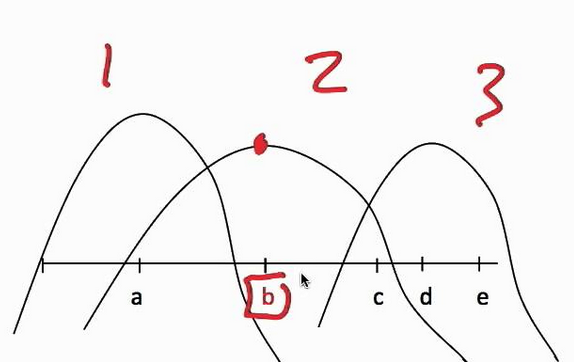
\includegraphics[scale=0.5]{sp.png}
     \end{center}
\end{frame}

%@@@@@@@@@@@@@@@@@@@@@@@@@@@@@@@@@@@@@@@@@@@@@@@@@
\begin{frame}
\frametitle{Example of a Theory: Spatial Voting}
\begin{itemize}
\item Can we offer predictions about what policy a group of rational actors will choose?
\bigskip
\bigskip
\item Median Voter Theorem: if preferences are single peaked and voting is by majority rule then there is a median voter and the winning alternative will be that preferred by the median voter.
\end{itemize}
    \begin{center}
     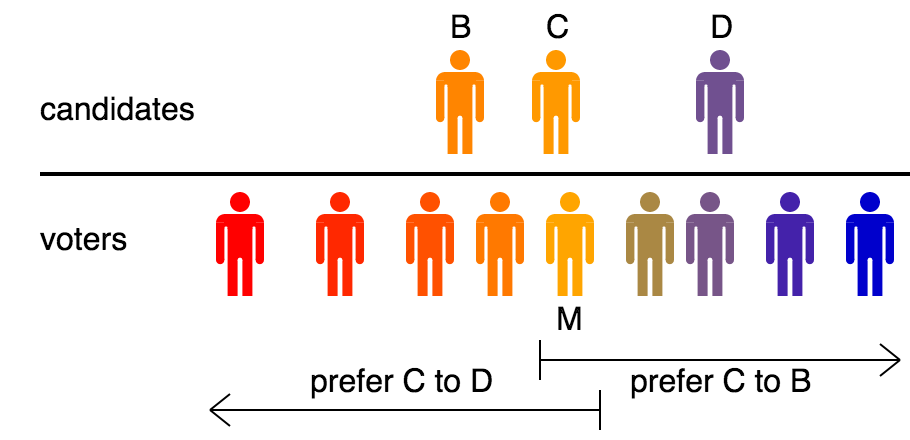
\includegraphics[scale=0.25]{Median_voter.png}
     \end{center}
\end{frame}

%@@@@@@@@@@@@@@@@@@@@@@@@@@@@@@@@@@@@@@@@@@@@@@@@@
\begin{frame}
\frametitle{The Logic of Science}
\begin{itemize}
\item If theory $T$ is true then hypotheses $H_1, H_2,\hdots$ are true (implication);
\bigskip
\bigskip
\item If hypothesis $H_1$ is true then test implications $I_1,I_2,\hdots$ are true (implication);
\bigskip
\bigskip
\item Example: 1854 London Cholera Outbreak;
\begin{itemize}
\item Severe cholera epidemic broke out in 1854 in London's Soho district -- 616 deaths;
\item Germ theory of disease: illness is caused by an unknown waterborne cell;
\item IF \textbf{germ theory} is true THEN \textbf{use of impure water spreads cholera};
\item IF \textbf{use of impure water spreads cholera} THEN \textbf{removing access will reduce cholera sickness/death rates};
\end{itemize}
\end{itemize}

\end{frame}

%@@@@@@@@@@@@@@@@@@@@@@@@@@@@@@@@@@@@@@@@@@@@@@@@@
\begin{frame}

\begin{center}
\includegraphics[scale=0.2]{Snow-cholera-map-1.jpg}
\end{center}

\end{frame}

%@@@@@@@@@@@@@@@@@@@@@@@@@@@@@@@@@@@@@@@@@@@@@@@@@
\begin{frame}
\frametitle{The Logic of Science}
\begin{itemize}
\item \textbf{Test 1 -- The Broad Street Pump:}
\begin{center}
\begin{quote}
On proceeding to the spot, I found that nearly all the deaths had taken place within a short distance of the [Broad Street] pump...I had an interview with the Board of Guardians of St. James's parish, on the evening of Thursday, the 7th September, and represented the above circumstances to them. In consequence of what I said, the handle of the pump was removed on the following day.
\end{quote}
\end{center}
\bigskip
\item \textbf{Test 2 -- Who provides the water?}
\begin{itemize}
\item Southwark and Vauxhall, and Lambeth Waterworks drew from Thames -- poorly filtered/yucky!
\item New River and Chelsea Companies drew from Thames -- much better filtration;
\item Significant variation in water supplier = natural experiment with 300k subjects;
\end{itemize}
\bigskip
\item \textbf{Results:} cholera generally ceased a few days after switching to cleaner water sources.
\end{itemize}

\end{frame}

%@@@@@@@@@@@@@@@@@@@@@@@@@@@@@@@@@@@@@@@@@@@@@@@@@
\begin{frame}
\frametitle{So what can we learn?}
\begin{itemize}
\item Removing access reduced cholera/death rates -- what does this mean?  More generally, what if are \textbf{test implications} are true?  And what does `true' mean?
\bigskip
\item Propositional logic -- the fallacy of \textit{\textbf{affirming the consequent}}:
\begin{itemize}
\item If $P$ is true then $Q$ is true;
\item $Q$ is true;
\item Therefore $P$ is true.
\item[] \color{white}THIS IS WRONG!
\item[]
\end{itemize}
\bigskip
\item[]  \color{white}Propositional logic -- modus tollens:
\begin{itemize}
\item[] \color{white}If P then Q;
\item[] \color{white}Not Q;
\item[] \color{white}Therefore, not P.
\item[]
\item[]
 \end{itemize}
\end{itemize}

\end{frame}

%@@@@@@@@@@@@@@@@@@@@@@@@@@@@@@@@@@@@@@@@@@@@@@@@@
\begin{frame}
\frametitle{So what can we learn?}
\begin{itemize}
\item Removing access reduced cholera/death rates -- what does this mean?  More generally, what if are \textbf{test implications} are true?  And what does `true' mean?
\bigskip
\item Propositional logic -- the fallacy of \textit{\textbf{affirming the consequent}}:
\begin{itemize}
\item If I fall off a cliff then I will be dead;
\item I am dead;
\item Therefore I fell off a cliff.
\item \textbf{THIS IS WRONG!}
\item[]
\end{itemize}
\bigskip
\item[]  \color{white}Propositional logic -- modus tollens:
\begin{itemize}
\item[] \color{white}If P then Q;
\item[] \color{white}Not Q;
\item[] \color{white}Therefore, not P.
\item[]
\item[]
 \end{itemize}
\end{itemize}

\end{frame}

%@@@@@@@@@@@@@@@@@@@@@@@@@@@@@@@@@@@@@@@@@@@@@@@@@
\begin{frame}
\frametitle{So what can we learn?}
\begin{itemize}
\item Removing access reduced cholera/death rates -- what does this mean?  More generally, what if are \textbf{test implications} are true?  And what does `true' mean?
\bigskip
\item Propositional logic -- the fallacy of \textit{\textbf{affirming the consequent}}:
\begin{itemize}
\item If an animal is a great white shark then it is a carnivore;
\item This animal is a carnivore;
\item Therefore it is a great white shark.
\item \textbf{THIS IS WRONG!}
\item[]
\end{itemize}
\bigskip
\item[]  \color{white}Propositional logic -- modus tollens:
\begin{itemize}
\item[] \color{white}If P then Q;
\item[] \color{white}Not Q;
\item[] \color{white}Therefore, not P.
\item[]
\item[]
 \end{itemize}
\end{itemize}

\end{frame}

%@@@@@@@@@@@@@@@@@@@@@@@@@@@@@@@@@@@@@@@@@@@@@@@@@
\begin{frame}
\frametitle{So what can we learn?}
\begin{itemize}
\item Removing access reduced cholera/death rates -- what does this mean?  More generally, what if are \textbf{test implications} are true?  And what does `true' mean?
\bigskip
\item Propositional logic -- the fallacy of \textit{\textbf{affirming the consequent}}:
\begin{itemize}
\item If germ theory is true then removing access to impure water will reduce cholera sickness/death rates;
\item Removing access to impure water DID reduce cholera sickness/death rates;
\item Therefore germ theory is true.
\item \textbf{THIS IS WRONG!}
\end{itemize}
\bigskip
\item[]  \color{white}Propositional logic -- modus tollens:
\begin{itemize}
\item[] \color{white}If P then Q;
\item[] \color{white}Not Q;
\item[] \color{white}Therefore, not P.
\item[]
\item[]
 \end{itemize}
\end{itemize}

\end{frame}

%@@@@@@@@@@@@@@@@@@@@@@@@@@@@@@@@@@@@@@@@@@@@@@@@@
\begin{frame}
\frametitle{So what can we learn?}
\begin{itemize}
\item Removing access reduced cholera/death rates -- what does this mean?  More generally, what if are \textbf{test implications} are true?  And what does `true' mean?
\bigskip
\item Propositional logic -- the fallacy of \textit{\textbf{affirming the consequent}}:
\begin{itemize}
\item If germ theory is true then removing access to impure water will reduce cholera sickness/death rates;
\item Removing access to impure water DID reduce cholera sickness/death rates;
\item Therefore germ theory is true.
\item \textbf{THIS IS WRONG!}
\end{itemize}
\bigskip
\item Propositional logic -- \textit{\textbf{modus tollens}}:
\begin{itemize}
\item If P then Q;
\item Not Q;
\item Therefore, not P.
\item[]
\item[]
 \end{itemize}
\end{itemize}

\end{frame}

%@@@@@@@@@@@@@@@@@@@@@@@@@@@@@@@@@@@@@@@@@@@@@@@@@
\begin{frame}
\frametitle{So what can we learn?}
\begin{itemize}
\item Removing access reduced cholera/death rates -- what does this mean?  More generally, what if are \textbf{test implications} are true?  And what does `true' mean?
\bigskip
\item Propositional logic -- the fallacy of \textit{\textbf{affirming the consequent}}:
\begin{itemize}
\item If germ theory is true then removing access to impure water will reduce cholera sickness/death rates;
\item Removing access to impure water DID reduce cholera sickness/death rates;
\item Therefore germ theory is true.
\item \textbf{THIS IS WRONG!}
\end{itemize}
\bigskip
\item Propositional logic -- \textit{\textbf{modus tollens}}:
\begin{itemize}
\item If Watson is a miniature schnauzer then Watson is a dog;
\item Watson is not a dog;
\item Therefore, Watson is not a miniature schnauzer.
\item[]
\item[]
 \end{itemize}
\end{itemize}

\end{frame}

%@@@@@@@@@@@@@@@@@@@@@@@@@@@@@@@@@@@@@@@@@@@@@@@@@
\begin{frame}
\frametitle{So what can we learn?}
\begin{itemize}
\item Removing access reduced cholera/death rates -- what does this mean?  More generally, what if are \textbf{test implications} are true?  And what does `true' mean?
\bigskip
\item Propositional logic -- the fallacy of \textit{\textbf{affirming the consequent}}:
\begin{itemize}
\item If germ theory is true then removing access to impure water will reduce cholera sickness/death rates;
\item Removing access to impure water DID reduce cholera sickness/death rates;
\item Therefore germ theory is true.
\item \textbf{THIS IS WRONG!}
\end{itemize}
\bigskip
\item Propositional logic -- \textit{\textbf{modus tollens}}:
\begin{itemize}
\item IF theory $T$ is true THEN hypothesis $H_1$ is true;
\item IF hypothesis $H_1$ is true THEN test implication $I_1$ is true;
\item Test implication $I_1$ is not true;
\item Therefore hypothesis $H_1$ is not true;
\item Therefore Theory $T$ is not true.
 \end{itemize}
\end{itemize}

\end{frame}

%@@@@@@@@@@@@@@@@@@@@@@@@@@@@@@@@@@@@@@@@@@@@@@@@@
\begin{frame}
\frametitle{Doctrine of Falsification}
\begin{itemize}
\item So what do we have?
\begin{enumerate}
\item Scientific theory is linked to the observable world by logical implication...
\item Affirming the consequent is a logical fallacy...
\item and \textit{modus tollens} allows us to show theories are false...
\end{enumerate}
\bigskip
\bigskip
\item We can never show theories to be true via empirical tests -- we can only show that either:
\begin{enumerate}
\item they are not inconsistent with the observable world or...
\item ...they are false.
\end{enumerate}
\bigskip
\bigskip
\item This is known as the \textbf{Falsifiability criterion} -- a cornerstone of science.
\end{itemize}

\end{frame}

%@@@@@@@@@@@@@@@@@@@@@@@@@@@@@@@@@@@@@@@@@@@@@@@@@
\begin{frame}

\begin{center}
\Huge\textbf{Why should we care?}\\
\bigskip
\bigskip
\large Everything else that follows is constrained by this logic -- we need to understand the limitations of the models we build and the things we can derive from them to use them properly.\\
\end{center}

\end{frame}

%ADD ONE MORE EXAMPLE

\end{document}






